\section{Теоретические и математические основы}

Пусть задан ориентированный граф $G = (V, E)$, где $V$~--- множество вершин, а $E$~--- множество направленных рёбер. Для описания топологии взвешенного ориентированного графа применяется матрица смежности $A$. В~формуле~(\ref{eq:adjacency}) представлено математическое определение элементов этой матрицы с~учётом весовой функции $w: E \to \mathbb{R}$:
\begin{equation}
A_{i,j} = \begin{cases} 
w(v_i, v_j), & \text{если } (v_i, v_j) \in E, \\ 
0, & \text{если } i = j, \\ 
\infty, & \text{в~противном случае.} 
\end{cases}
\label{eq:adjacency}
\end{equation}

Примеры топологических структур ориентированных графов приведены на рисунках~\ref{fig:graph1} и~\ref{fig:graph2}.

\begin{figure}[htbp]
    \centering
    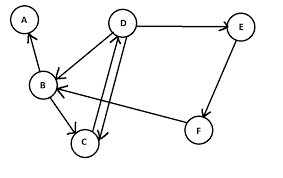
\includegraphics[width=0.5\textwidth]{graph1.png}
    \caption{Структурная схема ориентированного графа $G_1$}
    \label{fig:graph1}
\end{figure}

\begin{figure}[htbp]
    \centering
    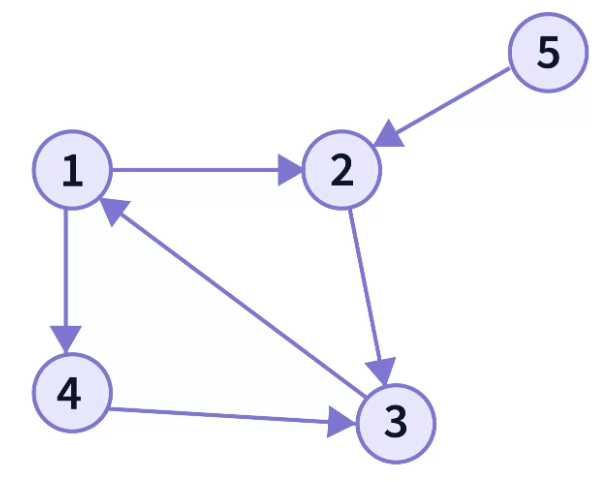
\includegraphics[width=0.5\textwidth]{graph2.png}
    \caption{Структурная схема ориентированного графа $G_2$}
    \label{fig:graph2}
\end{figure}

Поиск кратчайших путей является одной из~наиболее важных задач теории графов~\cite{henrick2017ml}. При наличии рёбер с~отрицательным весом классический алгоритм Дейкстры неприменим, и~вместо него используется уравнение Беллмана-Форда. Формула~(\ref{eq:bellman}) выражает шаг релаксации расстояния до вершины $v$ на итерации $k$:
\begin{equation}
d^{(k)}(v) = \min \left( d^{(k-1)}(v), \min_{u \in V} \left( d^{(k-1)}(u) + w(u, v) \right) \right)
\label{eq:bellman}
\end{equation}

В~случае отсутствия циклов отрицательного веса для любой вершины $v$, отличной от стартовой $s$, выполняется условие оптимальности, представленное в~формуле~(\ref{eq:optimality}):
\begin{equation}
\forall v \in V \setminus \{s\}: d(v) = \min_{u \in V: (u,v) \in E} \left\{ d(u) + w(u, v) \right\}
\label{eq:optimality}
\end{equation}

Сравнительные характеристики временной и~пространственной сложности основных алгоритмов обхода и поиска путей приведены в~таблице~\ref{tab:complexity}.

\begin{table}[htbp]
    \caption{Сравнительная сложность алгоритмов на графах}
    \label{tab:complexity}
    \begin{tabular}{|l|c|c|l|}
        \hline
        Алгоритм & Сложность по времени & Сложность по памяти & Ограничения \\
        \hline
        Обход в ширину (BFS) & $O(V + E)$ & $O(V)$ & Без весов рёбер \\
        Алгоритм Дейкстры & $O(E \log V)$ & $O(V)$ & Неотрицательные веса рёбер \\
        Алгоритм Беллмана-Форда & $O(V \cdot E)$ & $O(V)$ & Любые веса рёбер \\
        \hline
    \end{tabular}
\end{table}

\subsection{Практическая реализация алгоритма обхода графа}

Для анализа эффективности обхода ориентированных структур данных на практике была разработана программная реализация алгоритма поиска в~глубину (DFS) на~языке программирования C++.

В~качестве структуры представления графа был выбран список смежности на~основе вектора векторов \texttt{std::vector}. Это позволяет оптимально расходовать оперативную память и~выполнять операции обхода за линейное время $O(V + E)$. Для отслеживания посещённых вершин применяется вектор булевых значений \texttt{std::vector<bool>}.

Программный код разработанного алгоритма представлен в~листинге~\ref{code:dfs_code}.

\begin{listing}[htbp]
    \caption{Реализация алгоритма поиска в глубину (DFS) на C++}
    \label{code:dfs_code}
    \inputminted{text}{code.cpp}
\end{listing}
